\documentclass{beamer}
\mode<presentation>{\usetheme{Custom}}

\usepackage[orientation=portrait,size=a0,scale=1.4,debug]{beamerposter}
\usepackage[french]{babel}
\usepackage[utf8]{inputenc}
\usepackage{graphicx}
\usepackage{xcolor}
\usepackage{tcolorbox}
\usepackage{tikz}
\usepackage{tipa}

\tikzset{every picture/.style={execute at begin picture={
   \shorthandoff{:;!?};}
}}

\tikzset{rndblock/.style={rounded corners,rectangle,draw,outer sep=0pt}}
\newcommand{\tframed}[2][]{\tikz[baseline=0.1pt]\vspace{0.1cm}\node[rndblock,minimum height=1.5em,#1] (m) {#2} ;}
\newcommand{\hilight}[1]{\textbf{\tframed[blue,fill=blue!10]{#1}}}
\newcommand{\whilight}[1]{\textbf{\tframed[purple,fill=purple!10]{#1}}}


\newcommand{\sP}{\hspace{1pt}}
\newcommand{\mP}{\hspace{3pt}}
\newcommand{\bP}{\hspace{6pt}}
\newcommand{\BP}{\hspace{12pt}}

\definecolor{OrangeRed}{RGB}{255, 40, 0}
\definecolor{darksalmon}{RGB}{233,150,122}
\definecolor{blendedblue}{rgb}{0.137,0.466,0.741}
\definecolor{blendedgray}{rgb}{0.838,0.833,0.833}
\definecolor{blendedpurple}{RGB}{75,20,130}
\definecolor{tgray}{rgb}{0.211, 0.211,0.244}
\definecolor{darkgray}{rgb}{0.450,0.450,0.450}
\definecolor{maroon}{rgb}{0.695, 0.142, 0.142}
\definecolor{ngreen}{rgb}{0.000,0.500,0.000}
\definecolor{dgreen}{RGB}{0,150, 0}

\newcommand*{\TakeFourierOrnament}[1]{{%
\fontencoding{U}\fontfamily{futs}\selectfont\char#1}}
\newcommand*{\danger}{\TakeFourierOrnament{66}}


%%%%%%%%%%%%%%%%%%%%%%%%%%%%%%%%%%%%%%%%%%%%%%%%%%%%%%%%%%%%%%%%%%%%%%%%%%%%%%%%%%%%%%

\title{Reconnaissance de la parole pour l'aide à la communication \\pour les sourds et malentendants}
\author{Luiza Orosanu\\\vskip1.4ex Denis Jouvet}
\institute{Équipe PAROLE, Loria\\\vskip1.2ex Nancy, France}
\date[15 Octobre 2014]{15 Octobre 2014}

%%%%%%%%%%%%%%%%%%%%%%%%%%%%%%%%%%%%%%%%%%%%%%%%%%%%%%%%%%%%%%%%%%%%%%%%%%%%%%%%%%%%%%
\newlength{\columnheight}
\setlength{\columnheight}{105cm}


%%%%%%%%%%%%%%%%%%%%%%%%%%%%%%%%%%%%%%%%%%%%%%%%%%%%%%%%%%%%%%%%%%%%%%%%%%%%%%%%%%%%%%
\begin{document}
\begin{frame}


% ---------------------------------------------------------%
% Set up a row : introduction
% ---------------------------------------------------------%

\vskip0.3ex
\begin{beamercolorbox}[center,wd=\textwidth]{}
\begin{minipage}[T]{\textwidth}
\parbox[t][]{\textwidth}
{
	\begin{block}{Objectif global du projet RAPSODIE}

	\begin{columns}
	\begin{column}{.35\textwidth}
		Aider les \textbf{\color{OrangeRed} personnes sourdes ou malentendantes} \\
			{\small (améliorer la communication entre les sourds et leur entourage)}

		\vskip0.4ex
		\hskip15ex 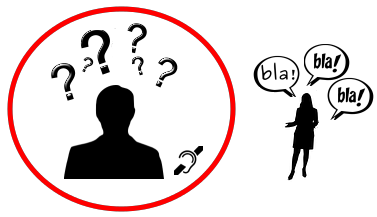
\includegraphics[scale=0.98]{Image/picture/deaf_support.png}

	\end{column}
	\begin{column}{.43\textwidth}
		Créer un système automatique de \textbf{\color{OrangeRed} transcription de la parole}

		\begin{center}
		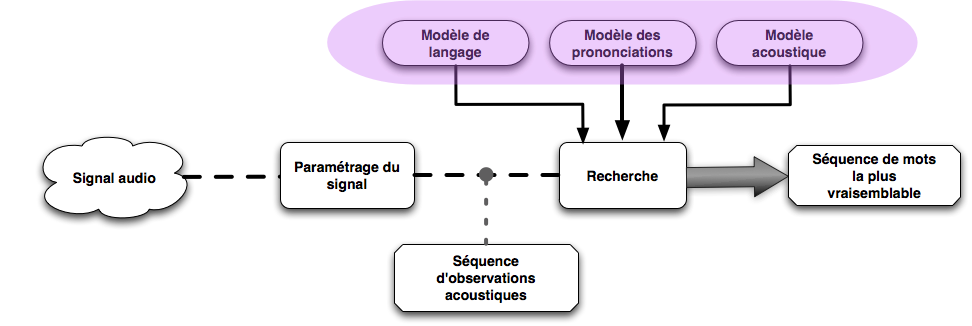
\includegraphics[scale=0.98]{Image/picture/rec2.png}
		\end{center}
	\end{column}
	\begin{column}{.18\textwidth}
		adapté aux contraintes imposés par une \\ \textbf{\color{OrangeRed} solution embarquée} : \\
			capacité mémoire \& puissance de calcul limitées
	\end{column}
	\end{columns}
	\end{block}

	%\item {\bf \color{OrangeRed} Approche}
	%\begin{itemize}
	%\item cibler seulement les personnes avec une bonne maitrise du Français écrit
	%\item faire des sacrifices par rapport à la taille de modèles de reconnaissance
	%\item prendre en compte les résultats des entretiens avec des personnes sourdes
	%\end{itemize}
}
\end{minipage}
\end{beamercolorbox}


\vskip0.5ex
\begin{columns}

% ---------------------------------------------------------%
% Set up a column
% ---------------------------------------------------------%

\begin{column}{.5\textwidth}
\begin{beamercolorbox}[center,wd=\textwidth]{postercolumn}
\begin{minipage}[T]{.985\textwidth}

\parbox[t][.7\columnheight]{\textwidth}
{
	\vskip0.5ex
	\begin{block}{Premier objectif : extraire des informations linguistiques}
		\begin{itemize}
			\item différentes unités linguistiques évaluées : mots, phonèmes, syllabes

				\vskip0.5ex
				\begin{center}
				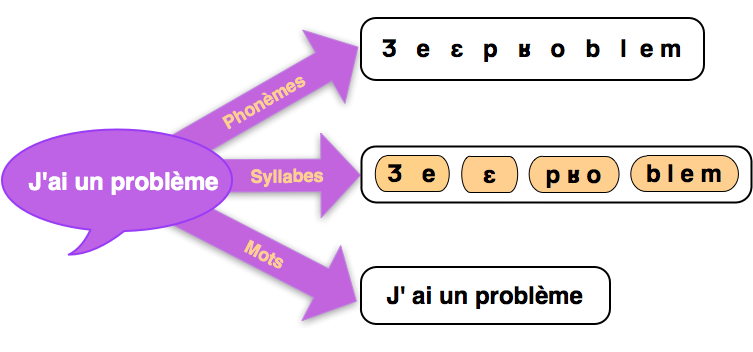
\includegraphics[scale=0.91]{Image/picture/select_LU.png}
				\end{center}
				$\rightarrow$ avec un lexique limité, les syllabes offrent des bonnes performances

			\vskip0.5ex
			\item à prendre en compte
				\begin{itemize}
				\item l'importance des mots pour la comprehension du message pour les sourds \\
				\item la problématique des mots hors de vocabulaire
				\end{itemize}

			\vskip0.5ex
			\item compromis : \textbf{combiner mots et syllabes} dans un seul modèle de langage
				\begin{itemize}
				\item assurer une reconnaissance correcte des mots les plus fréquents
				\item proposer des suites de syllabes pour les segments hors vocabulaire
				\end{itemize}
		\end{itemize}

		\vskip2ex
		{\color{blendedblue} \hrule }
		\vskip2ex

		\textbf{\color{OrangeRed} Création d'un modèle de langage hybride}
		\vskip.5ex

		\begin{itemize}
			\item constituer un corpus d'apprentissage qui repose sur ces deux unités lexicales
				\begin{itemize}
				\item conserver les mots les plus fréquents
				\item décomposer en syllabes les mots hors vocabulaire
				\end{itemize}

			\vskip1.8ex
			\item \textbf{Méthode pour définir les syllabes}
				\begin{itemize}
				\item corpus d'apprentissage entièrement phonétisé
					\begin{list}{\color{black!75} $\ast$}{\leftmargin=12mm \itemindent=0em}
					\item pour prendre en compte les événements de \textbf{\color{blendedblue} liaison \& réduction}
					\end{list}

				\vskip.5ex
				\item séquence de phonèmes traitée par des règles de syllabation \textbf{\footnotesize [Bigi et al, 2010]}
					\begin{list}{\color{black!75} $\ast$}{\leftmargin=12mm \itemindent=0em}
					\item une syllabe contient une seule voyelle
					\item une pause désigne une frontière de syllabe
					\end{list}
				\end{itemize}


				\begin{center}
				\hskip-3ex 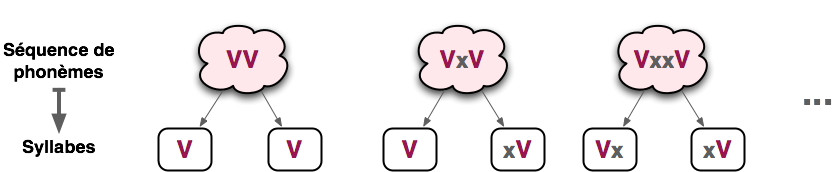
\includegraphics[scale=1.1]{Image/picture/syllabif.png}
				\end{center}

			\vskip1.8ex
			\item \textbf{Exemple d'une transcription "mots \& syllabes"}
		\end{itemize}

		\begin{table}[T]
		\begin{tabular}{lp{1cm}l}
	 	quel \bP est \bP le \bP  prix \bP  du  \bP \textbf{\color{maroon} tournevis} & & \\
		quel \bP est \bP le \bP  prix \bP  du  \bP \textbf{\color{maroon} t \sP u \sP r \sP n \sP \textschwa \bP \bP v \sP i \sP s} &  & \textbf{\color{blendedblue} $\leftarrow$ alignement forcé} \\
		quel \bP est \bP le \bP  prix \bP  du  \bP \textbf{\color{maroon} t\_u\_r \sP   n\_\textschwa \bP \bP \sP  v\_i\_s} 	 &  & \textbf{\color{blendedblue} $\leftarrow$ mots \& syllabes} \\
		\end{tabular}
		\end{table}

		\vskip1.5ex
		{\color{blendedblue} \hrule }
		\vskip2ex

		\textbf{\color{OrangeRed} Résultats }
		\vskip.5ex

		\begin{itemize}
			\item le modèle de langage hybride est un compromis efficace
			\item parmi les 69 à 96\% de mots qui sont reconnus par le système, environ 70\% d’entre eux sont effectivement correctement reconnus
			\item parmi les mots reconnus qui ont une mesure de confiance supérieure à 0.5, 85\% d'entre eux sont corrects
		\end{itemize}
	\end{block}
}

\end{minipage}
\end{beamercolorbox}
\end{column}

% ---------------------------------------------------------%
% Set up a column
% ---------------------------------------------------------%

\begin{column}{.5\textwidth}
\begin{beamercolorbox}[rounded=true,center,wd=\textwidth]{postercolumn}
\begin{minipage}[T]{.985\textwidth}
\parbox[t][.7\columnheight]{\textwidth}
{
	\vskip0.5ex
	\begin{block}{Deuxième objectif : extraire des informations complémentaires}
		\begin{itemize}
			\item détecter la modalité des énoncés : \textbf{\color{OrangeRed} question ou affirmation}
			\item dans un contexte interactif il est important de savoir si un message correspond à une question
			\item deux types de questions
				\begin{itemize}
				\item exprimées par des tournures interrogatives
				\item perçues comme des interrogations qu'au travers de la prosodie
			\end{itemize}
		\end{itemize}

		\vskip2ex
		{\color{blendedblue} \hrule }
		\vskip2ex

		\textbf{\color{OrangeRed} Méthodologie pour la détection de questions}
		\vskip.5ex

		\begin{itemize}
			\item évaluer plusieurs approches
			\begin{itemize}
				\item un classifieur prosodique : utilise la prononciation
				\item un classifieur linguistique : utilise les mots qui compose la phrase
				\item un classifieur combiné : utilise les informations prosodique et  linguistique
			\end{itemize}
		\end{itemize}

		\vskip1.5ex
		\begin{itemize}
			\item \textbf{Les paramètres linguistiques}
		\end{itemize}

		\begin{columns}
		\begin{column}{.76\textwidth}
			 \begin{list}{\color{black!75} $\triangleright$}{\leftmargin=22.5mm \itemindent=0em}
				\item les tournures interrogatives : pour indiquer la présence ou l'absence d'une tournure interrogative dans la phrase

				\vskip3ex
				\item la probabilité que la phrase soit une question

				$\ast$ par rapport à deux modèles de langage de référence

				%\begin{center}
				$$\text{LL(phrase)}=\text{Log}\left(\frac{\text{P(phrase} \rvert \text{ML-question)}}{\text{P(phrase} \rvert \text{ML-affirmation)}}\right)$$
				%\end{center}

				\vskip1ex
				$\ast$ LL $\geq$ 0  $\rightarrow$ susceptible d'être une question \\
				$\ast$ LL $\textless$ 0 $\rightarrow$ susceptible d'être une affirmation
			\end{list}
		\end{column}
		\begin{column}{.28\textwidth}
			\begin{center}
			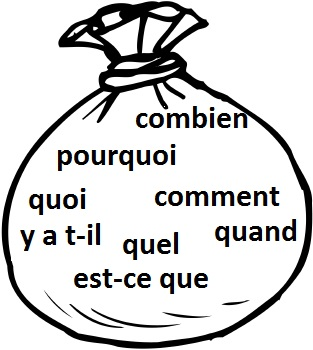
\includegraphics[scale=0.72]{Image/picture/motsInterrogatifs.jpg}
			\vskip1ex
			\hskip-3ex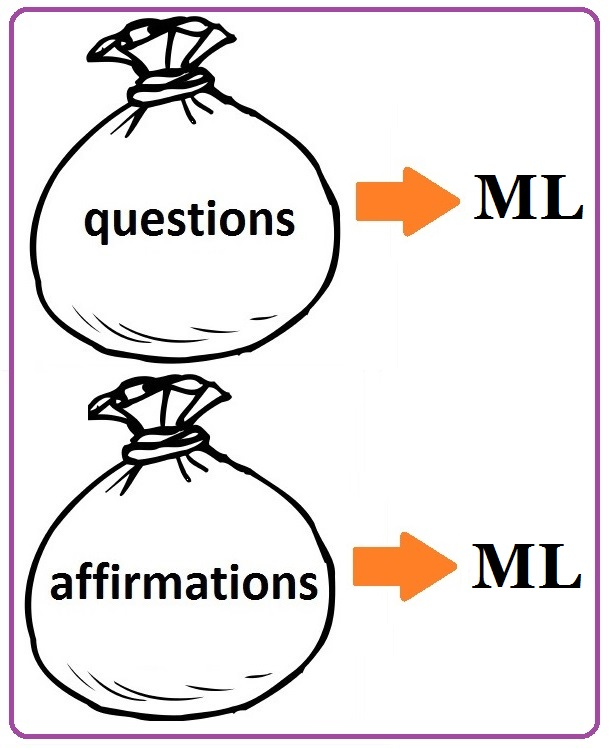
\includegraphics[scale=0.62]{Image/picture/lesMLs.jpg}
			\end{center}
		\end{column}
		\end{columns}

		\vskip2ex
		\begin{itemize}
			\item \textbf{Les paramètres prosodiques}
		\end{itemize}

		\begin{columns}
		\begin{column}{.45\textwidth}
			\begin{list}{\color{black!75} $\triangleright$}{\leftmargin=22.5mm \itemindent=0em}
				\item l'intonation d'une question comporte en général un pitch final montant
				\item 10 paramètres prosodiques qui prennent en compte la durée, l'énergie et le pitch du dernier groupe prosodique de la phrase
			\end{list}
		\end{column}
		\begin{column}{.54\textwidth}
			\begin{center}
			\hskip-2ex 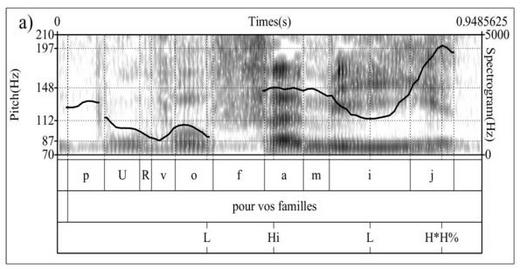
\includegraphics[scale=1.5]{Image/picture/prosodie.png}
			\end{center}
		\end{column}
		\end{columns}

		\vskip1.5ex
		\begin{itemize}
			\item \textbf{L'évaluation} est effectuée en utilisant des paramètres linguistiques issus des transcriptions \textbf{manuelles} et \textbf{automatiques}
		\end{itemize}

		\vskip1.5ex
		{\color{blendedblue} \hrule }
		\vskip2.5ex

		\textbf{\color{OrangeRed} Résultats }
		\vskip.5ex

		\begin{itemize}
			\item l'essentiel de l'information pour la détection de la modalité des énoncés provient du contenu linguistique de l'énoncé
			\item lorsque l'on se place dans un contexte applicatif (transcription automatique), les performances du détecteur linguistique baissent,
				et la prosodie apporte un complément d'information significatif
		\end{itemize}

	\end{block}
}
\end{minipage}
\end{beamercolorbox}
\end{column}
\end{columns}


% ---------------------------------------------------------%
% Set up a row : conclusions & future work
% ---------------------------------------------------------%

\vskip8.5ex
\begin{beamercolorbox}[center,wd=\textwidth]{}
\begin{minipage}[T]{\textwidth}
\parbox[t][]{\textwidth}
{
	\begin{block}{Travaux futurs}
		\begin{columns}
		\begin{column}{.49\textwidth}
			\begin{itemize}
				\item étudier d'autres solutions pour mieux modéliser les syllabes à l'intérieur d'un modèle hybride
				\item analyser les segments correspondants aux mots hors vocabulaire
			\end{itemize}
		\end{column}
		\begin{column}{.49\textwidth}
			\begin{itemize}
				\item étudier plus les caractéristiques prosodiques et linguistiques
				\item prendre en compte les mesures de confiance dans le calcul des paramètres linguistiques
			\end{itemize}
		\end{column}
		\end{columns}
	\end{block}
}
\end{minipage}
\end{beamercolorbox}

\end{frame}
\end{document}

